\subsection*{Formula}
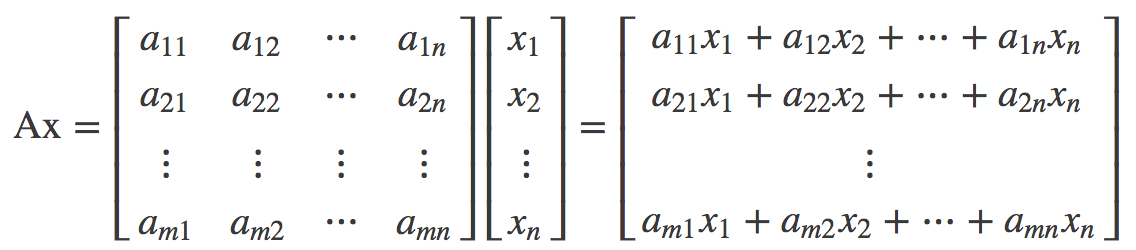
\includegraphics[width=\linewidth]{matmul.png}
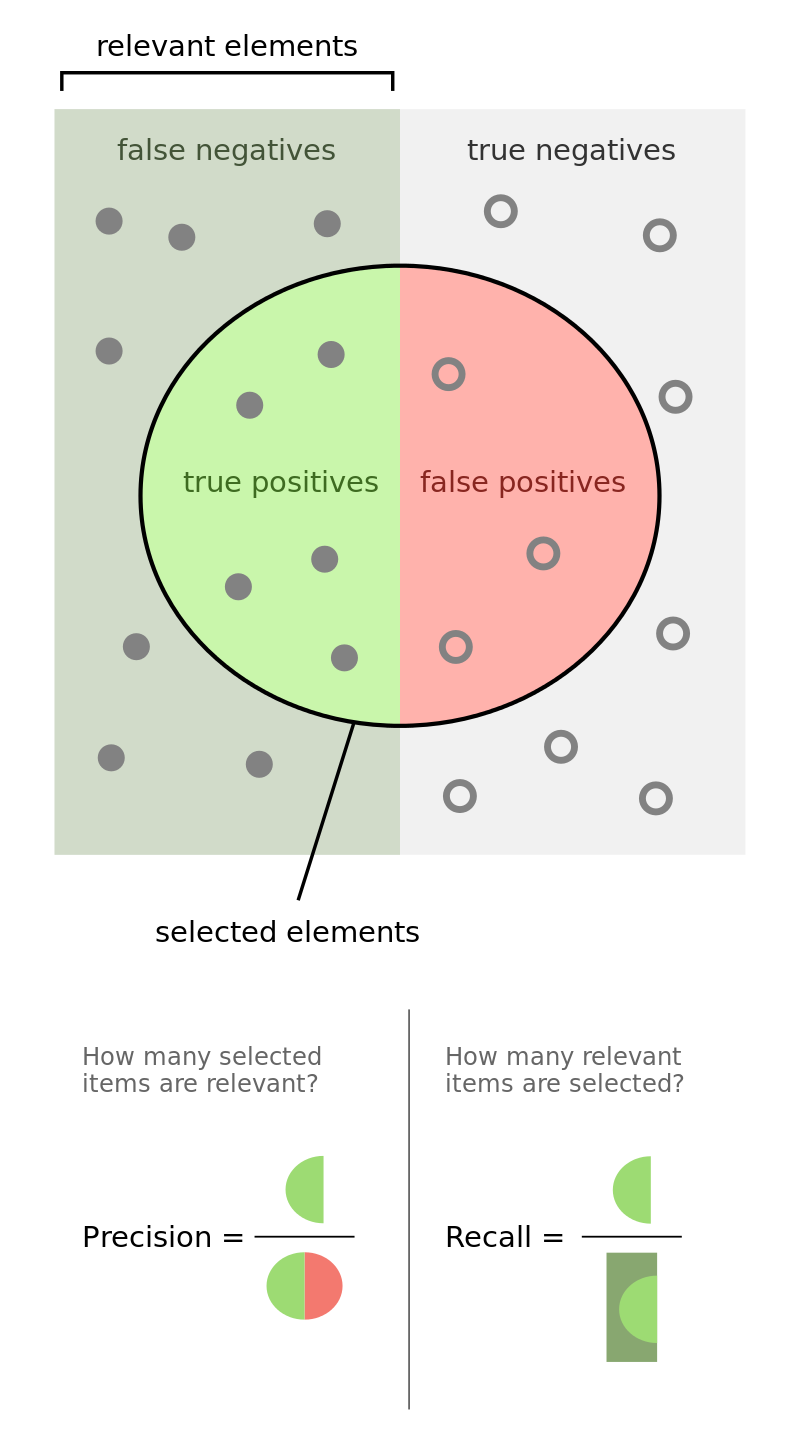
\includegraphics[width=\linewidth]{precisionrecall.png}

sigmoid: $\frac{1}{1+e^{-x}}$
\\
sigmoid drv: $\sigma(1-\sigma)$
\\
tanh drv: $1-tanh^2(x)$

\subsection*{Batch Norm}
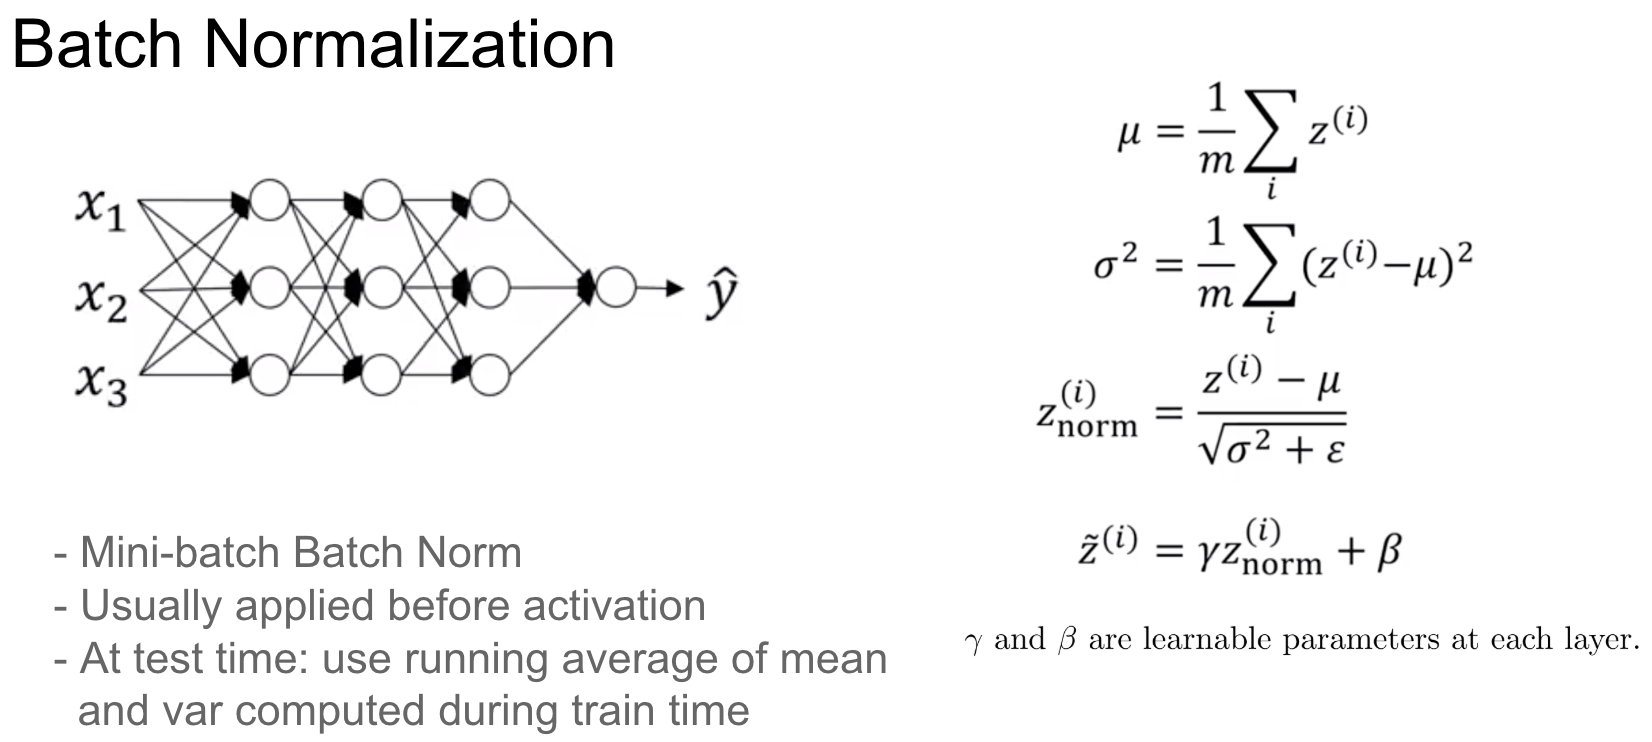
\includegraphics[width=\linewidth]{batchnorm.png}
(i) accelerates learning by reducing covariate shift, decoupling dependence of layers, and/or allowing for higher learning rates/ deeper networks, (ii) accelerates learning by normalizing contours of output dis- tribution to be more uniform across dimensions, (iii) Regularizes by using batch
To receive full credit, these responses included three components: (i) Mini-batches might be small at test time. (ii) Smaller mini-batches mean the mini-batch statistics are more likely to differ from the mini-batch statistics used at training. (iii) Moving averages are better estimates.

\subsection*{Optimizers}
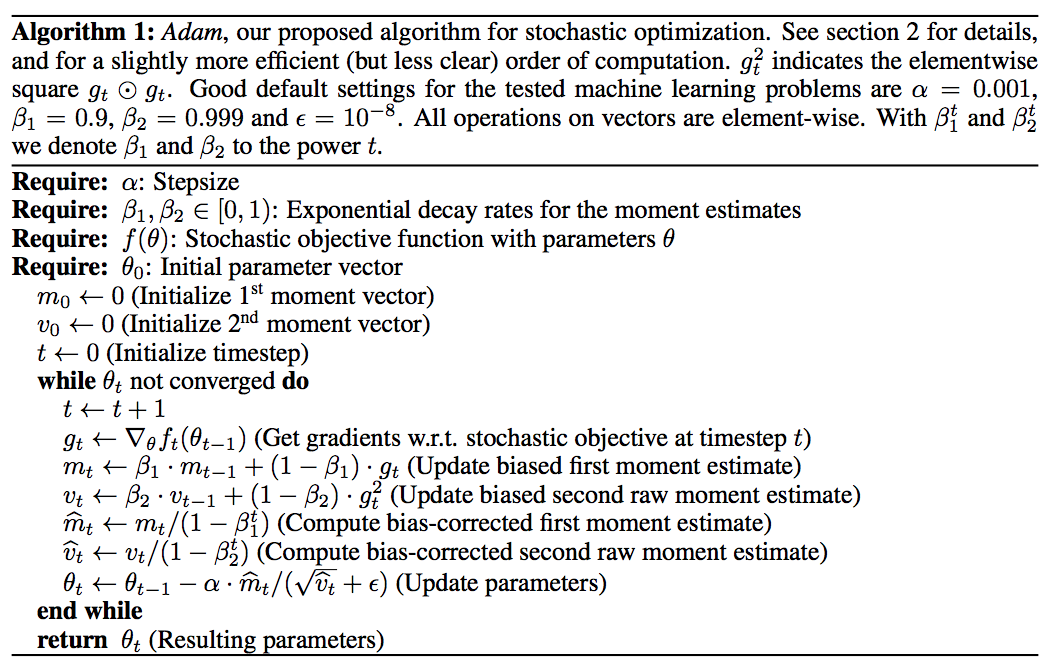
\includegraphics[width=\linewidth]{adam.png}
There are a few important differences between RMSProp with momentum and Adam: RMSProp with momentum generates its parameter updates using a momentum on the rescaled gradient, whereas Adam updates are
directly estimated using a running average of first and second moment of the gradient. RMSProp
also lacks a bias-correction term; this matters most in case of a value of β2 close to 1 (required in
case of sparse gradients), since in that case not correcting the bias leads to very large stepsizes and
often divergence,

\subsection*{Backprop}
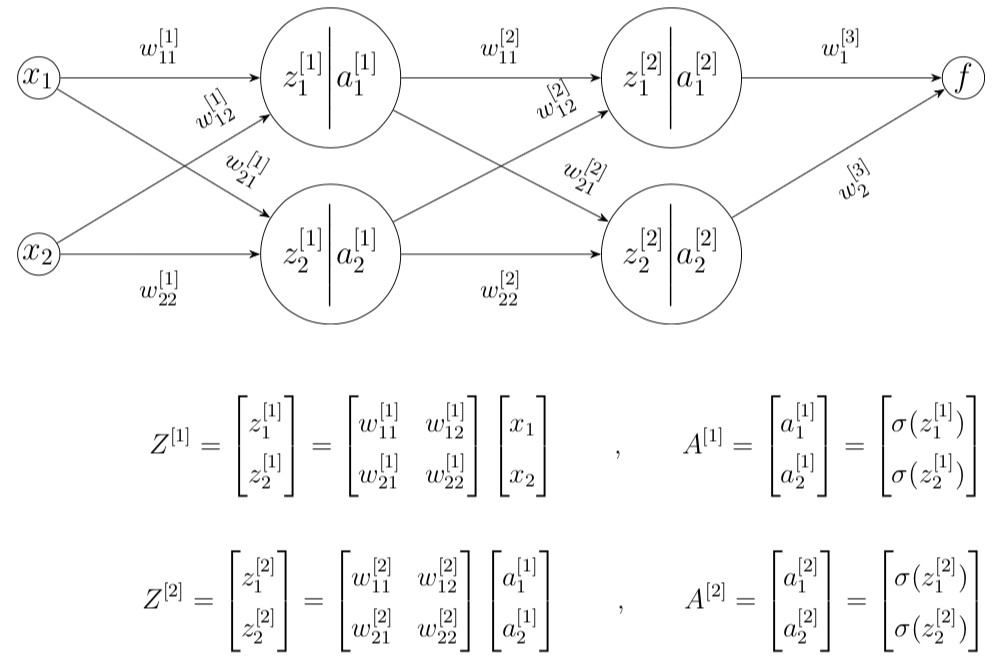
\includegraphics[width=\linewidth]{network.png}
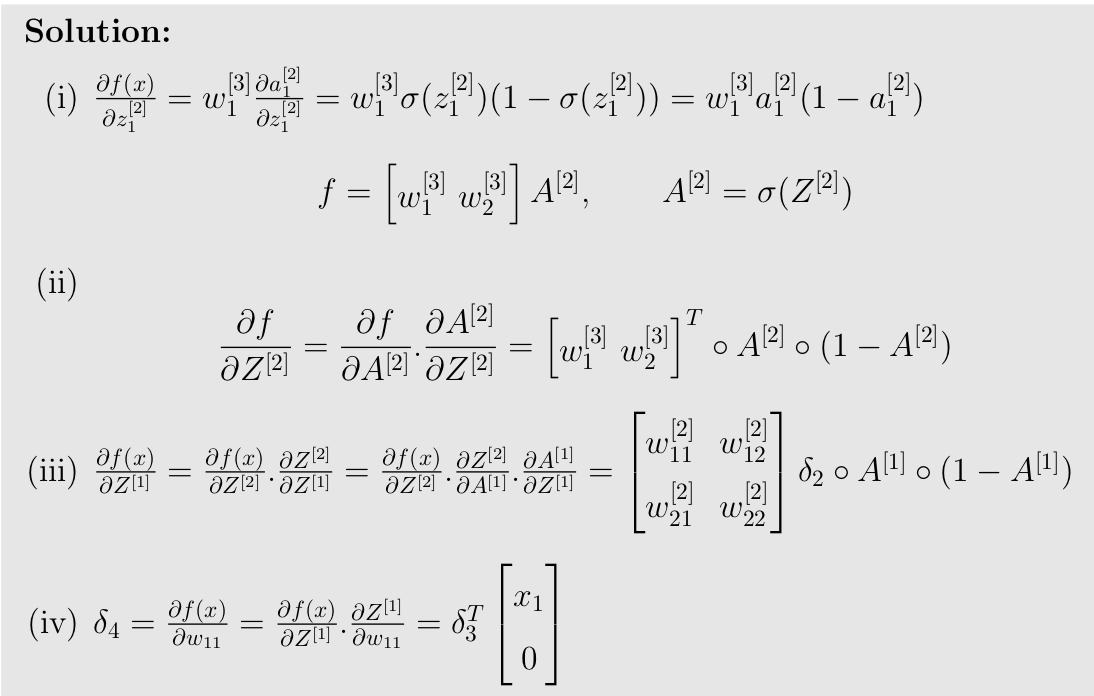
\includegraphics[width=\linewidth]{network_sol.png}

\subsection*{GAN}
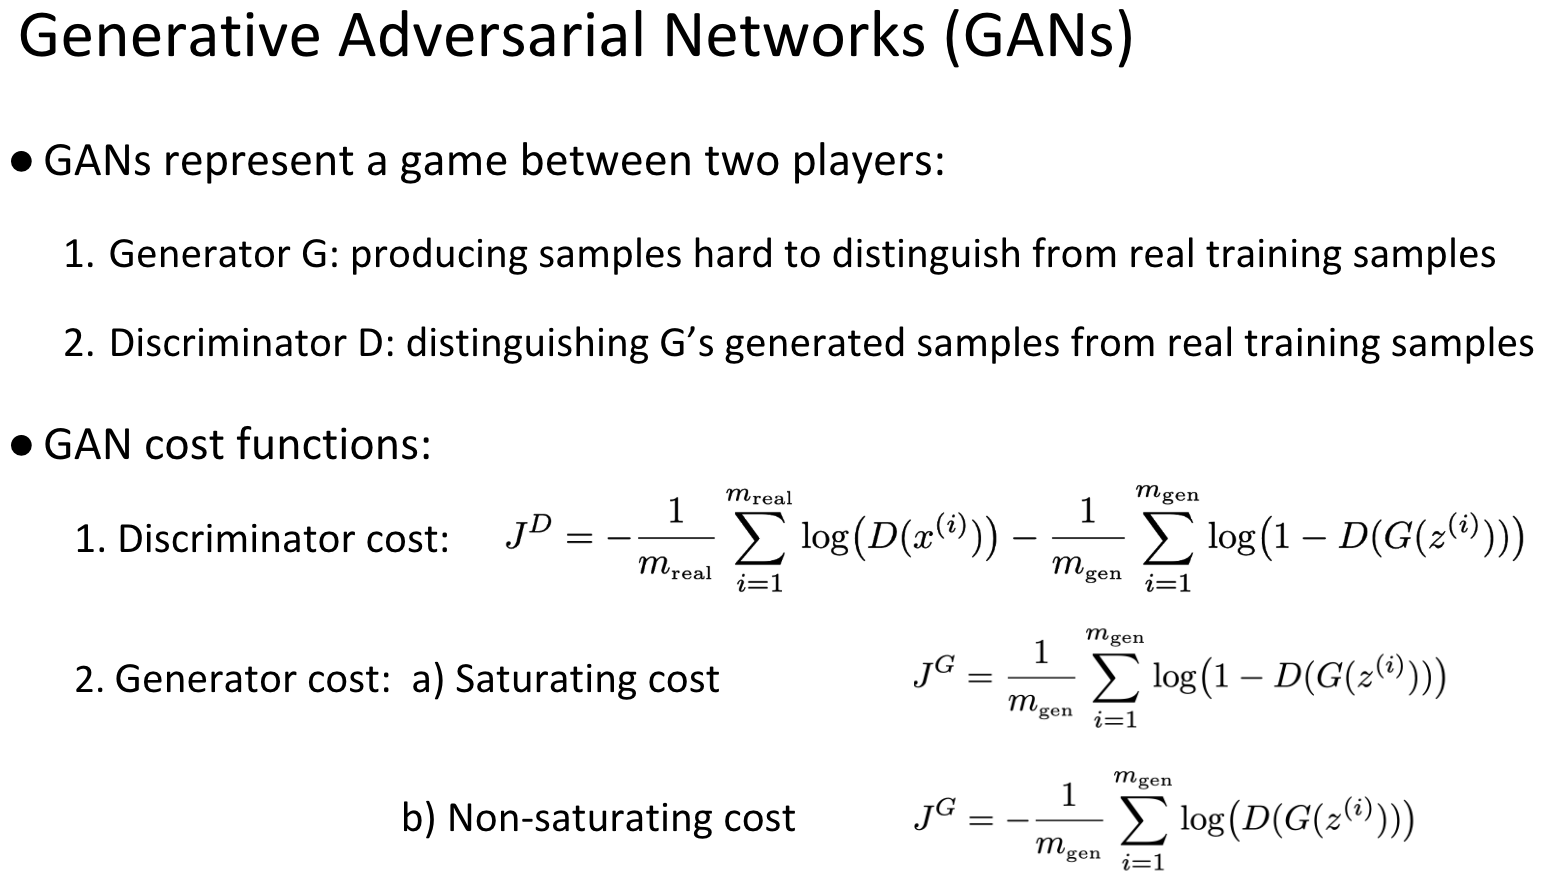
\includegraphics[width=\linewidth]{gan.png}

\subsection*{CNN}
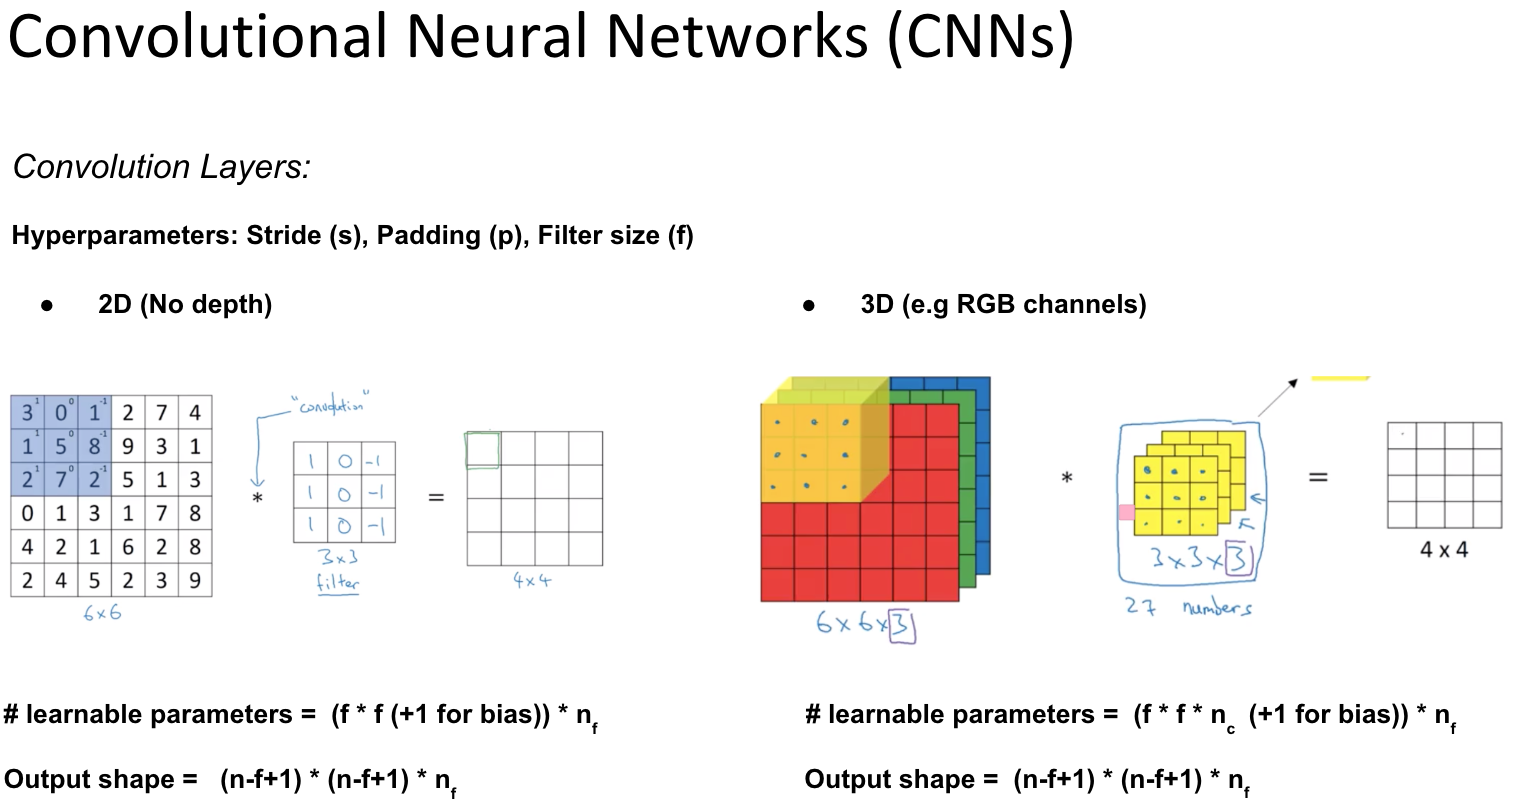
\includegraphics[width=\linewidth]{cnn1.png}
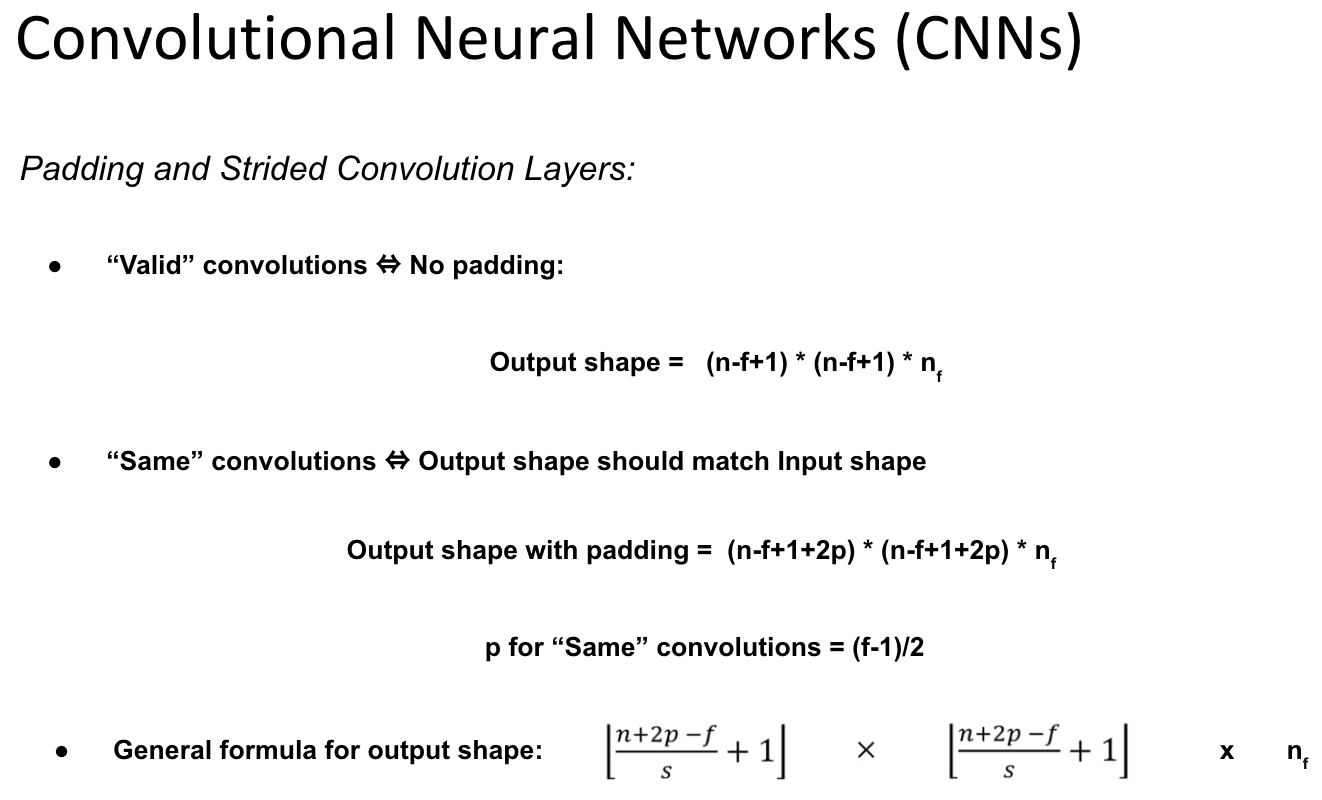
\includegraphics[width=\linewidth]{cnn2.png}
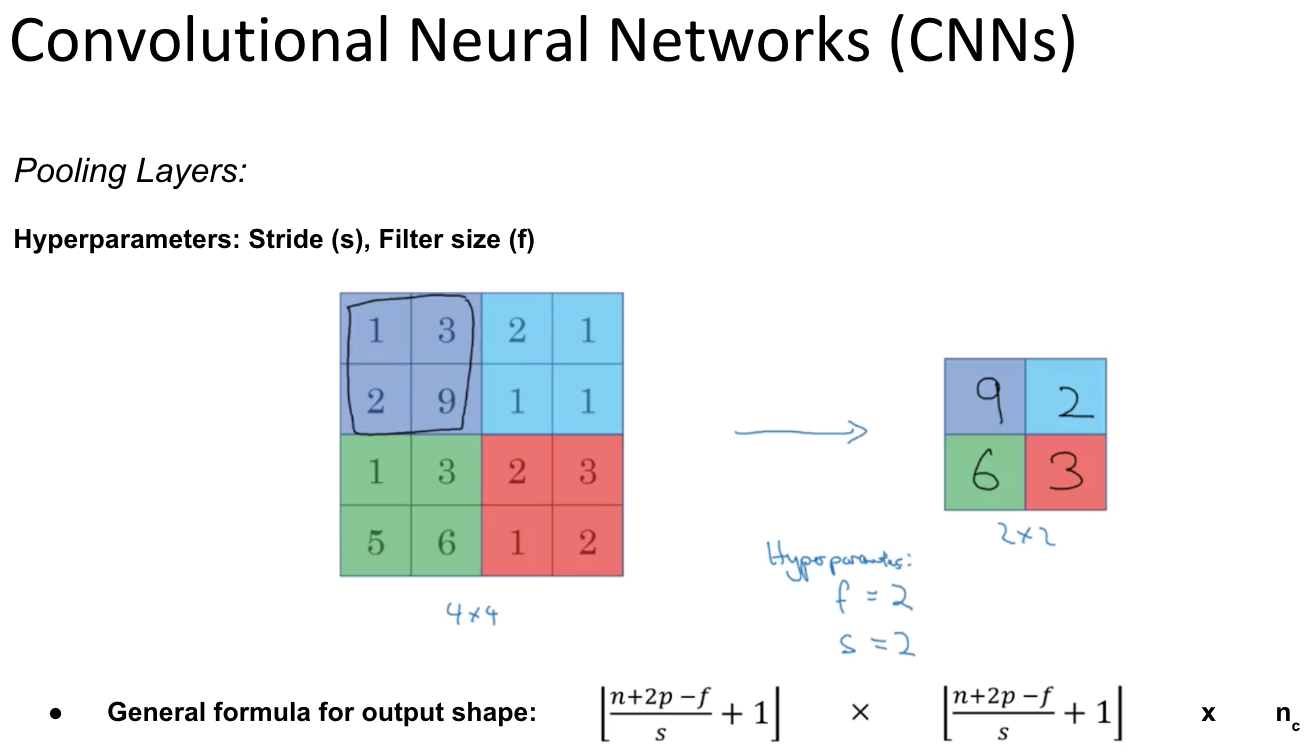
\includegraphics[width=\linewidth]{cnn3.png}

\subsection*{Dropout}
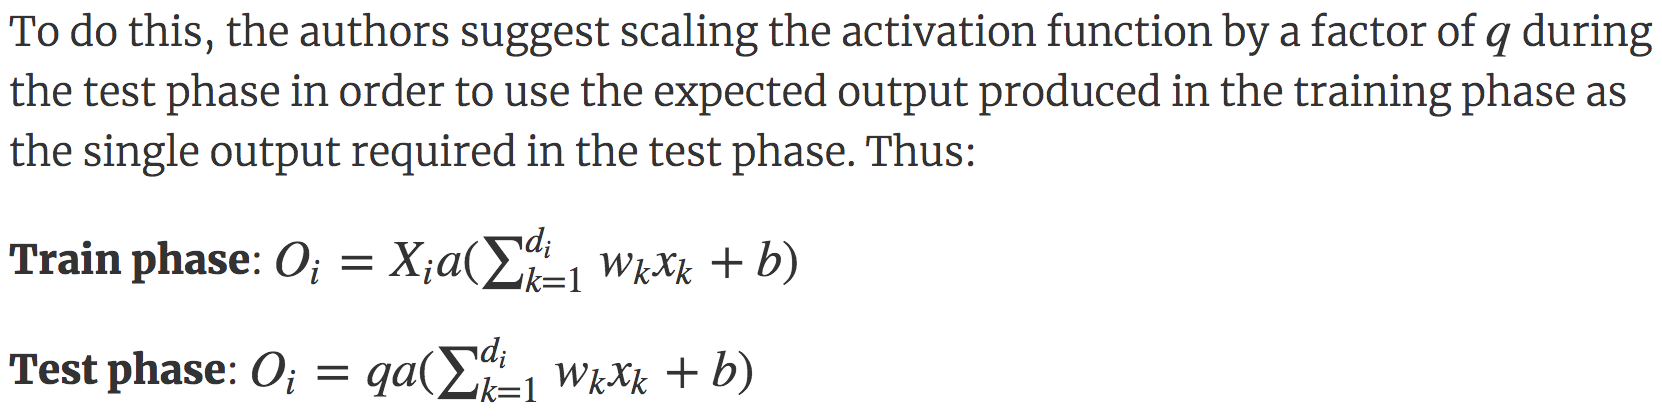
\includegraphics[width=\linewidth]{dropout.png}
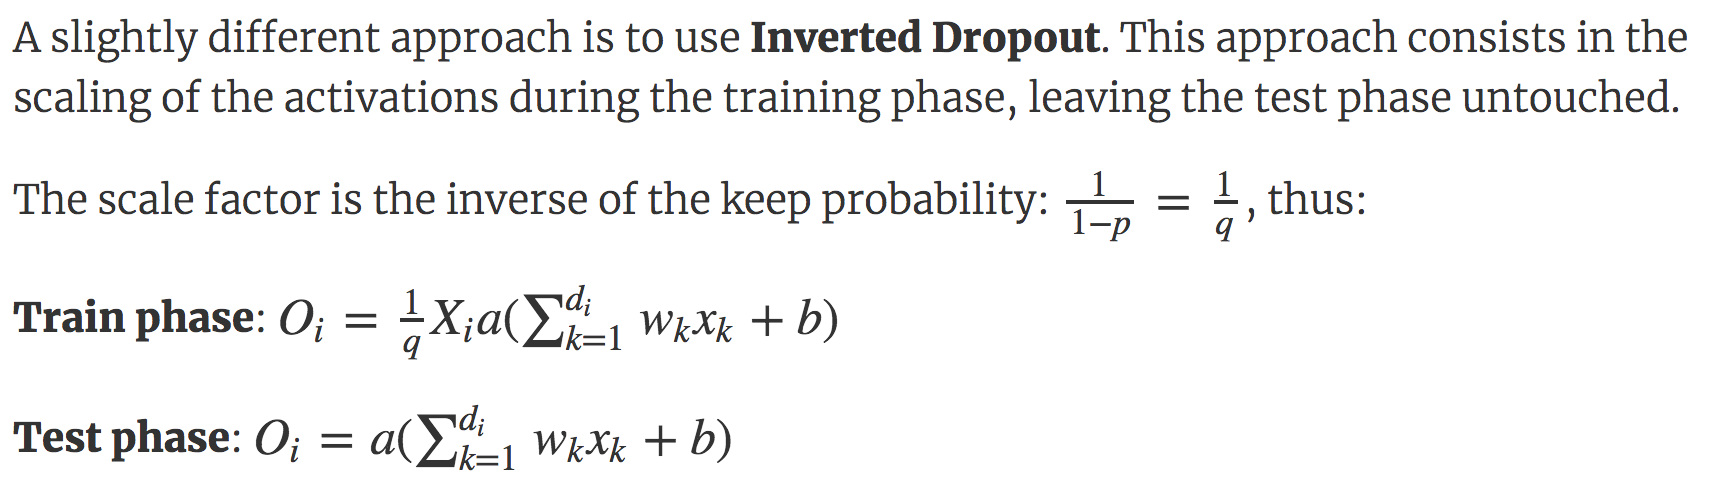
\includegraphics[width=\linewidth]{invdropout.png}

\subsection*{Bias}
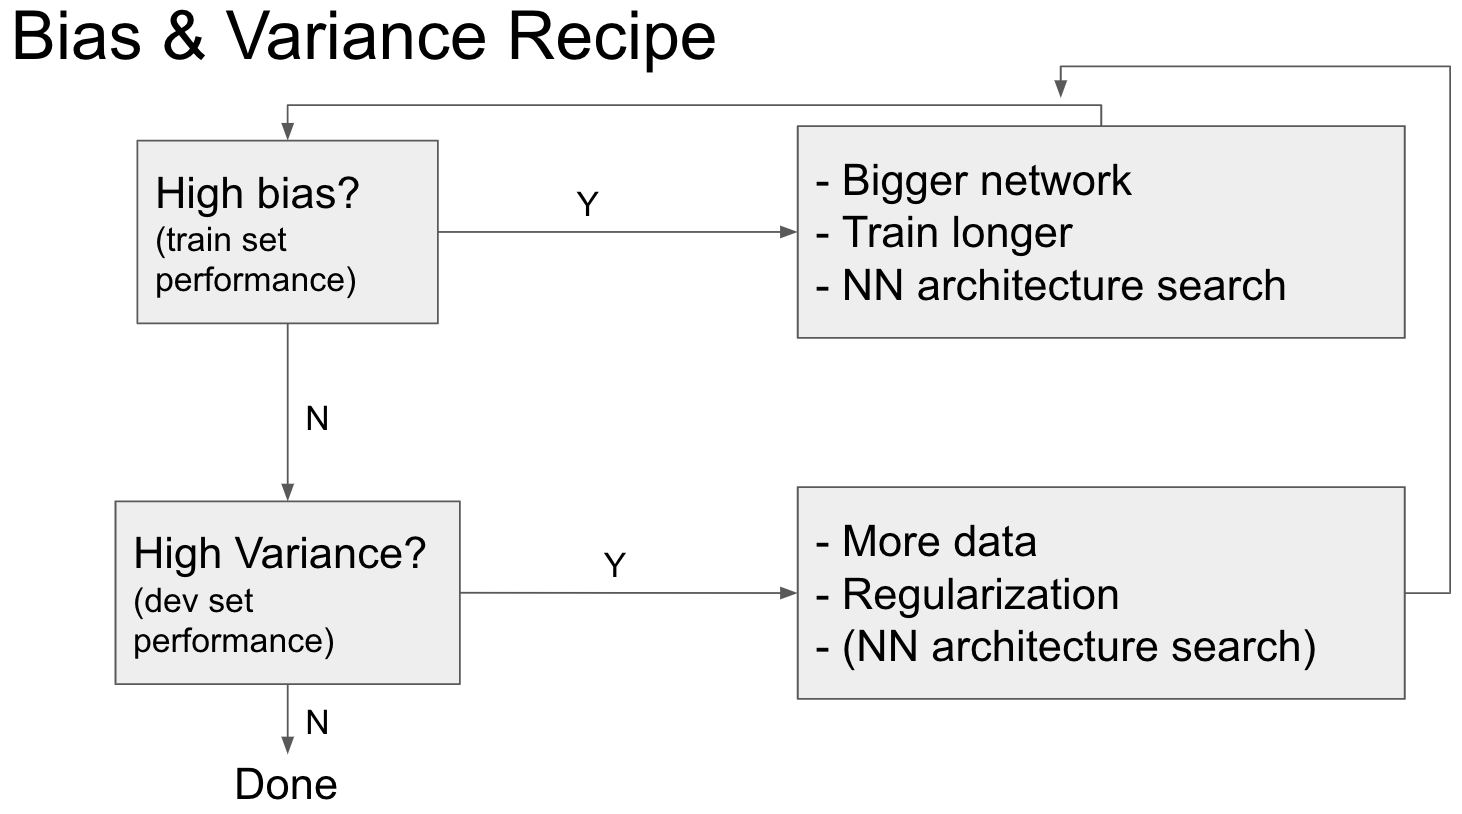
\includegraphics[width=\linewidth]{biasvar.png}

